\section{Using HTML, CSS \& JavaScript}\label{sec:todo}

\subsection{Project}

\subsubsection*{Project Description}

This is a minimal To-do List application written in HTML, CSS and JavaScript. It is a single page application that allows the user to add, edit and delete tasks.

The tasks are added though a form that is displayed at the top of the page.
The tasks are displayed in an unordered list below the form. And a delete button is displayed next to each task.
The click and submit events are handled by JavaScript functions.

\subsubsection*{Project Showcase}

\begin{figure}[H]
    \centering
    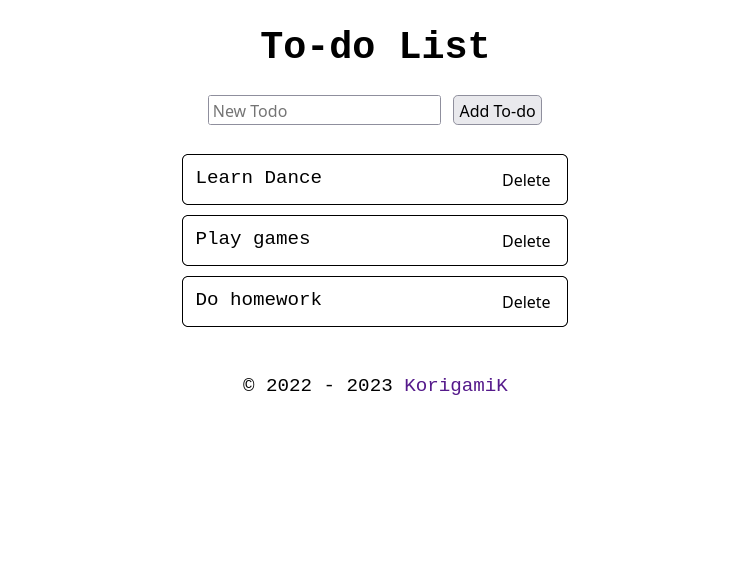
\includegraphics[width=0.8\textwidth]{res/todo-list.png}
    \caption{To-do List App}
    \label{fig:todo-list}
\end{figure}


\subsection{Source Code}

File: \texttt{todo-list.html}
\htmlcode{./code/todo-list.html}
